\section{Data Life Cycle}

Throughout the literature, a variety of different definitions of data life cycle models can be found. Although they have been developed for different actuation domains, we describe here some of them which we think that can be applied for generic data, independently of its original domain.

\subsection{Data Documentation Initiative}

The first model to be analysed is the model proposed by Data Documentation Initiative (DDI). The DDI introduced a Combined Life Cycle Model for data managing \cite{data_documentation_initiative_overview_2008}. As Figure \ref{fig:ddi} shows, this model has eight elements or steps which can be summarized as follows, according to \cite{ball_review_2012}:

\begin{itemize}
    \item \textbf{Study Concept.} At this stage, apart from choosing the research question and the methodology for collecting the data, also plans the processing and analysis of data to answer the question.
    \item \textbf{Data Collection.} This model proposes different methods to collect data, like surveys, health records, statistics or Web-based collections.
    \item \textbf{Data Processing.} At this stage, the collected data is processed to answer the proposed research question. The data may be recorded both machine-readable and human-readable form.
    \item \textbf{Data Archiving.} Both data and metadata should be archived to ensure long-term access to them, ensuring the confidentiality.
    \item \textbf{Data Distribution.} This stage involves the different ways which the data are distributed and questions related to terms of use of the data or citation of the original sources. 
    \item \textbf{Data Discovery.} The data may be published in different manners, through publications, web-indexes, etc.
    \item \textbf{Data Analysis.} The data can be used by others to achieve different goals.
    \item \textbf{Repurposing.} The data can be used outside of their original framework, restructuring them or combining with different data.
\end{itemize}

%TODO: Vectorialize
\begin{figure}
    \center
    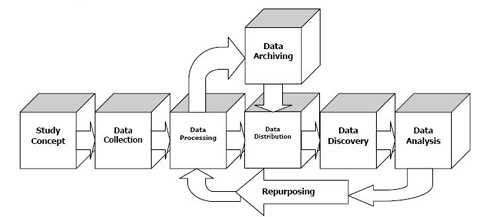
\includegraphics[width=\textwidth]{img/data_lifecycle/what-is-ddi-diagram.jpg}
    \caption{Combined Life Cycle Model (ownership: DDI Alliance).}
    \label{fig:ddi}
\end{figure}

%\footnotetext{\url{http://www.ddialliance.org/}}

\subsection{Australian National Data Service}

In late 2007 the Australian National Data Service (ANDS) was founded with the target of creating a national data management environment. ANDS established a set of verbs, denominated Data Sharing Verbs that describe the entire life cycle of the data \cite{burton_designing_2009}:

\begin{itemize}
    \item \textbf{Create.} \textit{Create} (or \textit{collect} for disciplines with an observational focus) is about the kinds of metadata that could be collected and the tools for fulfill this collection task.
    \item \textbf{Store.} This \textit{Sharing Verb} remarks the need for stable and web-accessible storage, taking care about the appropriate storing of data.
    \item \textbf{Describe.} The more information is inside the storage, more difficult is its discovery, access and exploit. Annotating the data with the proper metadata solves this issue.
    \item \textbf{Identify.} The application of this verb implies the proper identification of each data resource, assigning a persistent identifier to each of them.
    \item \textbf{Register.} This Verb pertains to registering the descriptions of the different data collections with one or more public catalogues.
    \item \textbf{Discover.} To improve the data-reusing, ANDS suggests to enable different discovery services.
    \item \textbf{Access.} To guarantee the appropriate access to data, ANDS suggests to provide a suitable search engine to retrieve these data. If the data is not electronically available, ANDS recommends to provide contact details to get the data in conventional forms.
    \item \textbf{Exploit.} \textit{Exploit}, the final Data Verb, involves the tools, methodologies and support actions to enable reutilisation of data.
\end{itemize}

\subsection{Ecoinformatics data life cycle}

Michener and Jones define in \cite{michener_ecoinformatics:_2012} the concept of ``ecoinformatics'': \textit{a framework that enables scientists to generate new knowledge through innovative tools and approaches for discovering, managing, integrating, analysing, visualizing and preserving relevant biological, environmental, and socioeconomic data and information.} To manage these data, the following data life cycle has been defined, as can be seen at Figure \ref{fig:ecoinformatics}:
\begin{itemize}
    \item \textbf{Plan.} This step involves the confection of a data management planning.
    \item \textbf{Collect.} This step consider both manual (hand-written data sheets) and automatic (sensor networks) data-collection methods.
    \item \textbf{Assure.} Quality assurance and quality control (QA/QC), an issue which in previously mentioned models is not taken into account, refers to developing methods to guarantee the integrity of the data. Quality assurance also can consists of defining standards for formats, codes, measurement units, metadata, etc.
    \item \textbf{Describe.} As other data life cycle models, this model remarks the value of the metadata to answer to questions about \textit{who, when, where, how} and \textit{why}.
    \item \textbf{Preserve.} Data preservation implies the storage of the data and metadata, ensuring that these data can be verified, replicated and actively curated over time.
    \item \textbf{Discover.} The authors describe the data discover as \textit{one of the greatest challenges}, as many data are not immediately available because there are stored in individual laptops. The main challenges to publish the data in a proper way are related about the creation of catalogues and indexes, and about the implementation of the proper search engines.
    \item \textbf{Integrate.} Integrating data from different and heterogeneous sources can become into a difficult task because it requires \textit{understanding methodological differences, transforming data into a common representation, and manually converting and recording data to compatible semantics before analysis can begin}.
    \item \textbf{Analyze.} As well as the importance of a clear analysis, this models remarks the importance of documenting this analysis with sufficient detail to enable its reproduction in different research frameworks.
\end{itemize}

\begin{figure}
    \center
    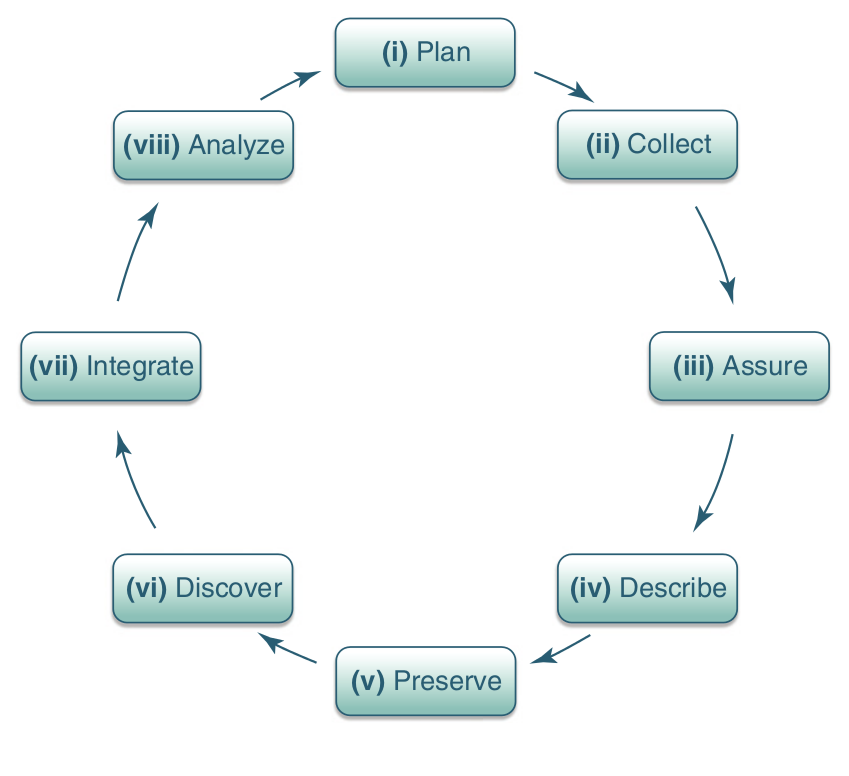
\includegraphics[scale=0.3]{img/data_lifecycle/ecoinformatics.png}
    \caption{Data life cycle in ecoinformatics. Taken from \cite{michener_ecoinformatics:_2012}.}
    \label{fig:ecoinformatics}
\end{figure}

\subsection{UK Data Archive}

The last analyzed data life cycle model, is the one proposed by UK Data Archive\footnote{\url{http://www.data-archive.ac.uk/create-manage/life-cycle}}. This model is oriented to help researchers to publish their data in a manner which allows other researchers continuing their work independently. In Figure \ref{fig:uk-data-archive}, we can observe the following stages:
\begin{itemize}
    \item \textbf{Creating data.} Creating the data involves the design of the research question, planning data management and their sharing. If we want to reuse existing data, we have to locate existing data and collect these data. As well as the data is new or is an existing data, at this stage the metadata has to be created.
    \item \textbf{Processing data.} Like in other models, at this stage the data is translated, checked, validated and cleaned. In the case of the confidential data, they have to be ``anonymized''. The UK Data Archive recommends to create the metadata at this stage too.
    \item \textbf{Analysing data.} At this stage the data are interpreted and derived into visualizations or reports. In addition, the data are prepared for preservation, as can be seen at following stage.
    \item \textbf{Preserving data.} To preserve the data properly, they are migrated to the best format and stored in a suitable medium. In addition to the previously created metadata, the creating, processing, analysis and preserving process are documented.
    \item \textbf{Giving access to data.} Once the data is stored, we have to distribute our data. This distribution of the data may involve controlling the access to them and establish a sharing license.
    \item \textbf{Re-using data.} At last, the data can be re-used enabling new research topics.
\end{itemize}

\begin{figure}
    \center
    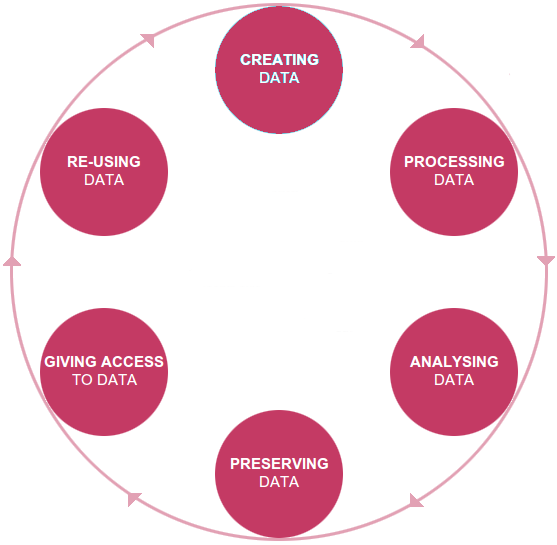
\includegraphics[scale=0.4]{img/data_lifecycle/uk-data-archive.png}
    \caption{Data life cycle proposed by UK Data Archive.}
    \label{fig:uk-data-archive}
\end{figure}

\subsection{A common data life cycle for smart cities}
